\documentclass[dvipdfmx,tikz]{standalone}
\usepackage{tikz}
\usetikzlibrary{intersections,calc,arrows}
\begin{document}
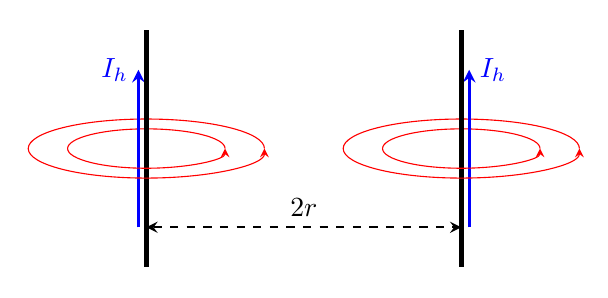
\begin{tikzpicture}
%\draw[help lines] (-3,-2) grid (3,2);

\draw[line width=2pt] (-2,-1.5) -- (-2,0);
\draw[line width=2pt] (2,-1.5) -- (2,0);

\draw[line width=1pt,color = blue] (-2.1,-1) -- (-2.1,0);
\draw[line width=1pt,color = blue] (2.1,-1) -- (2.1,0);

\draw[->,>=stealth,color = red] (-1,0) arc [start angle=0, end angle=360,x radius=1, y radius=0.25];
\draw[->,>=stealth,color = red] (-0.5,0) arc [start angle=0, end angle=360,x radius=1.5, y radius=0.375];

\draw[->,>=stealth,color = red] (3,0) arc [start angle=0, end angle=360,x radius=1, y radius=0.25];
\draw[->,>=stealth,color = red] (3.5,0) arc [start angle=0, end angle=360,x radius=1.5, y radius=0.375];

\draw[->,>=stealth,line width=1pt,color = blue] (-2.1,0) -- (-2.1,1) node[anchor = east] {$I_h$};
\draw[->,>=stealth,line width=1pt,color = blue] (2.1,0) -- (2.1,1) node[anchor = west] {$I_h$};

\draw[line width=2pt] (-2,0) -- (-2,1.5);
\draw[line width=2pt] (2,0) -- (2,1.5);
\draw[<->,>=stealth,thick,dashed] (-2,-1) -- (2,-1) node[midway,above] {$2r$};
\end{tikzpicture}
\end{document}